\documentclass[aps,prd,twocolumn,showpacs,superscriptaddress,nofootinbib]{revtex4-2}

\usepackage{amsmath,amssymb}
\usepackage{graphicx}
\usepackage{booktabs}
\usepackage{siunitx}
\usepackage{hyperref}

% Canonical counts pipeline (Phase 5v: freshness gate).
% Auto-generated by update_counts.py — 2026-11-05T17:29:00.839938
% Do not edit manually. Run: uv run python scripts/update_counts.py
\newcommand{\leantoolchain}{4.32.0}
\newcommand{\mathlibrev}{81a5d257}
\newcommand{\physlibrev}{c4843367}
\newcommand{\totaltheorems}{30948}
\newcommand{\substantivetheorems}{30922}
\newcommand{\placeholdertheorems}{26}
\newcommand{\kernelsubstantivetheorems}{30853}
\newcommand{\trackedvacuitydebt}{69}
\newcommand{\axiomcount}{0}
\newcommand{\sorrycount}{0}
\newcommand{\sorrypercent}{0.0}
\newcommand{\leanmodules}{2152}
\newcommand{\leandefinitions}{15467}
\newcommand{\pythonmodules}{140}
\newcommand{\testfiles}{218}
\newcommand{\totaltests}{8140}
\newcommand{\figurecount}{170}
\newcommand{\notebookcount}{91}
\newcommand{\papercount}{42}
\newcommand{\aristotleproved}{313}
\newcommand{\aristotleruns}{40}
% --- D11 bundle substrate summary (source-level, stated rule) ---
\newcommand{\dxiModules}{22}
\newcommand{\dxiLines}{6267}
\newcommand{\dxiTheorems}{403}
\newcommand{\dxiDefs}{82}
\newcommand{\dxiDepsTheorems}{409}
% --- Paper 18 / Phase 5t per-section counts (FermiHubbardDimer.lean) ---
\newcommand{\fhdTotal}{130}
\newcommand{\fhdWaveTwo}{13}
\newcommand{\fhdWaveThree}{6}
\newcommand{\fhdWaveFour}{19}
\newcommand{\fhdWaveFive}{20}
\newcommand{\fhdWaveSixABC}{35}
\newcommand{\fhdWaveSixExtra}{13}
\newcommand{\fhdWaveSeven}{17}
\newcommand{\fhdWaveEight}{7}
% --- Paper 26 / 27 per-module counts (BH entropy + four laws) ---
\newcommand{\bhEntropyTotal}{32}
\newcommand{\bhThermoTotal}{20}
% --- Phase 6 per-module + pytest counts (paper32 / paper34-38 / note_rt_ch_bounds) ---
\newcommand{\strongCpDeThms}{8}
\newcommand{\strongCpDeTests}{14}
\newcommand{\epThms}{24}
\newcommand{\epTests}{38}
\newcommand{\qecHolographyThms}{10}
\newcommand{\qecHolographyTests}{30}
\newcommand{\centerSymmThms}{18}
\newcommand{\centerSymmTests}{28}
\newcommand{\chiralSsbThms}{10}
\newcommand{\chiralSsbTests}{14}
\newcommand{\cflThms}{12}
\newcommand{\cflTests}{17}
\newcommand{\rtChThms}{7}
\newcommand{\rtChTests}{29}
\newcommand{\heatKernelThms}{20}
\newcommand{\heatKernelTests}{39}
\newcommand{\higherCurvatureThms}{13}
\newcommand{\higherCurvatureTests}{42}
\newcommand{\diffInvarianceThms}{13}
\newcommand{\diffInvarianceTests}{36}
\newcommand{\nonlinearEFEThms}{13}
\newcommand{\nonlinearEFETests}{40}
\newcommand{\microscopicCoefficientMatchThms}{12}
\newcommand{\microscopicCoefficientMatchTests}{42}
\newcommand{\einsteinCartanExtensionThms}{12}
\newcommand{\einsteinCartanExtensionTests}{41}
\newcommand{\bbnThms}{14}
\newcommand{\bbnTests}{16}
% --- Phase 6f/6g classical-GR per-module + wave totals (I1 §11–§13) ---
\newcommand{\curvatureThms}{14}
\newcommand{\einsteinTensorThms}{9}
\newcommand{\energyConditionsThms}{8}
\newcommand{\exactSolutionsThms}{16}
\newcommand{\admFormalismThms}{10}
\newcommand{\tetradFormalismThms}{5}
\newcommand{\phaseSixfWonesixTotal}{62}
\newcommand{\phaseSixfWsevenTotal}{13}
\newcommand{\riemannCoordinateThms}{8}
\newcommand{\riemannDifferentialBianchiThms}{8}
\newcommand{\bundleRiemannAuxThms}{6}
\newcommand{\bundleRiemannThms}{7}
\newcommand{\leviCivitaThms}{7}
\newcommand{\phaseSixfWeightTotal}{36}
\newcommand{\riccatiComparisonThms}{11}
\newcommand{\mazurSigmaModelRigidityThms}{12}
\newcommand{\hawkingPenroseCurveThms}{6}
\newcommand{\areaTheoremCurveThms}{10}
\newcommand{\phaseSixgWnineTotal}{39}
% --- D2 chirality-bundle per-module theorem counts (same convention as \totaltheorems) ---
\newcommand{\dtwoSmFermionDataThms}{19}
\newcommand{\dtwoZsixteenAnomalyThms}{23}
\newcommand{\dtwoVecGMonoidalThms}{11}
\newcommand{\dtwoToricCodeCenterThms}{25}
\newcommand{\dtwoCenterEquivalenceThms}{10}
\newcommand{\dtwoGoltermanShamirThms}{32}
\newcommand{\dtwoLatticeHamiltonianThms}{33}
\newcommand{\dtwoTpfEvasionThms}{14}
\newcommand{\dtwoPauliMatricesThms}{15}
\newcommand{\dtwoBdgHamiltonianThms}{8}
\newcommand{\dtwoChiralityWallMasterThms}{16}
\newcommand{\dtwoOnsagerAlgebraThms}{41}
\newcommand{\dtwoOnsagerContractionThms}{12}
\newcommand{\dtwoGtWeylDoubletThms}{15}
\newcommand{\dtwoFkGappedInterfaceThms}{12}
% --- paper10 per-module theorem counts (same convention as \totaltheorems) ---
\newcommand{\paperTenWangBridgeThms}{8}
\newcommand{\paperTenModularInvarianceThms}{11}
% --- Cross-platform Lean theorem reuse, 1+1D BEC -> 2+1D graphene (D1) ---
% Owner: scripts/count_theorem_reuse.py (population = the nine
% 1+1D BEC modules; REUSED = statement is platform-parametric).
\newcommand{\reuseTransferred}{107}
\newcommand{\reusePopulation}{120}
\newcommand{\reuseSpecific}{13}
\newcommand{\reusePercent}{89.17}
\newcommand{\reusePercentRounded}{89}
\newcommand{\reuseSpecificPercentRounded}{11}


\newcommand{\cGW}{c_{\rm GW}}
\newcommand{\chivest}{\chi_{\rm vest}}
\newcommand{\GammaH}{\Gamma_{H}}
\newcommand{\dccap}{\Delta c/c}
\newcommand{\GNemerg}{G_{N}^{\rm emerg}}
\newcommand{\Lambdauv}{\Lambda_{\rm UV}}
\newcommand{\Mpl}{M_{P}}
\newcommand{\Nf}{N_{f}}

\begin{document}

\title{A Conditional GW170817 Constraint on a Vestigial-Susceptibility Speed Law}

\author{John G.\ Roehm}
\affiliation{NetRxn Foundation}

\date{\today}

\begin{abstract}
For the assumed gravitational-wave speed law
$\cGW=c\sqrt{\chivest}$, the conservative symmetric GW170817
cap $|\dccap|\leq\tau$, with $\tau=3\times10^{-15}$,
is equivalent to
$\chivest\in[(1-\tau)^2,(1+\tau)^2]$.
This finite interval has center $1+\tau^2$, half-width $2\tau$
and width $4\tau$. It lies strictly inside the adopted comparison
range $[0.1,10]$ and occupies the fraction $4\tau/9.9$ of its width;
that fraction is not a probability without a specified prior.
The lower and upper comparison endpoints exceed the speed cap by
approximately $2.3\times10^{14}$ and $7.2\times10^{14}$,
respectively, while exact luminality occurs at $\chivest=1$.
We formalize the scalar identities, interval and endpoint results,
and four explicit counterexamples to the conjunction of positivity,
cap compatibility and sub-half relative deviation.
An illustrative frequency correction is an unmatched product ansatz;
its conditional placeholder bound supplies no physical detection band.
Neither the spin-two second-sound interpretation nor the
susceptibility-dependent speed law is derived from a microscopic
metric action here. The physical susceptibility normalization and
domain, propagating tensor mode, matter reference and controlled
transport remain required for a physical application.
The finite interval constrains this adopted law under the source-emission
assumptions used to infer the GW170817 cap; it excludes neither all
vestigial phases nor the emergent-gravity framework.
\end{abstract}

\pacs{04.30.-w, 04.50.-h, 04.20.-q, 04.60.-m, 04.80.Cc}

\maketitle

%% ================================================================
\section{Introduction}
\label{sec:intro}

Composite-tetrad gravity provides a setting for asking whether metric
order can precede a nonzero tetrad expectation.
Volovik's vestigial-phase proposal describes precisely such an
expectation-valued metric~\cite{Volovik2024Vestigial}.
A separate de~Sitter two-fluid calculation gives a collective
second-sound speed $s_2=c$~\cite{Volovik2026SecondSound}.
That work discusses possible graviton interpretations and leaves
the type of the collective mode open; it does not derive the
spin-two identification adopted here.

We assume both a spin-two interpretation of a candidate
metric-channel excitation and the kinematic law
$\cGW=c\sqrt{\chivest}$, where $\chivest$ is a free,
dimensionless normalized susceptibility. The RPA resummation
supplies a conditional response in terms of a bare susceptibility
and coupling, not a numerical physical value or a derivation of
this speed law. A quadratic action, constrained propagator,
tensor polarizations and matter coupling are still required.

The August 17, 2017 binary-neutron-star merger
(GW170817)~\cite{Abbott2017GW170817} placed an extraordinarily
tight bound on $\cGW$: by comparing the gravitational-wave arrival
time at LIGO/Virgo against the gamma-ray-burst signal at
Fermi/INTEGRAL, the multi-messenger collaboration constrained
$-3 \times 10^{-15} \leq (\cGW - c)/c \leq +7 \times 10^{-16}$.
We adopt the conservative symmetric envelope
$|\dccap| \leq 3 \times 10^{-15}$ under the collaboration's
distance and source-emission assumptions. Alternative emission histories
can weaken the inferred propagation constraint.

We formalize the consequences of the assumed speed law and
compare them with the conservative GW170817 envelope. For
$\cGW = c\,\sqrt{\chivest}$, compatibility requires a sub-interval of the adopted range $\chivest \in [0.1, 10]$
narrower than that range by $\sim 14$ orders
of magnitude. The GW170817-compatible window
$[(1-\tau)^{2}, (1+\tau)^{2}]$ has width exactly $4\tau$ in
$\chivest$ and lies strictly interior to $[0.1,10]$, containing the
anchor $\chivest=1$. Its relative width is $4\tau/9.9$; its
probability mass depends on the prior.

This is a conditional constraint on one specific kinematic
identification (second-sound mode = graviton). It excludes the two
natural-range endpoints under the assumed speed law while allowing
the finite interval above. The width comparison alone neither
refutes emergent gravity or the ADW program nor tests the
linearized-Einstein identification~\cite{Roehm2026LinearizedEFE}. Possible microscopic mechanisms are discussed in
Sec.~\ref{sec:discussion}.

%% ================================================================
\section{Setup}
\label{sec:setup}

\subsection{Vestigial-susceptibility identification}

The RPA resummation used in
\texttt{VestigialSusceptibility.lean} has the conditional closed form
$\chi_{\rm RPA}=\chi_0/(1-\gamma_\star\chi_0)$.
The bare susceptibility $\chi_0$ and effective coupling
$\gamma_\star$ are inputs; this formula does not evaluate them or
supply a normalized physical $\chivest$.
The comparison interval $\chivest\in[0.1,10]$ spans one decade
on either side of unity and is adopted, not calculated.
It is dimensionless. Deriving its physical normalization and
stable parameter domain requires the metric-channel source,
projector, regulator and microscopic response.
Vergeles's unitarity analysis~\cite{Vergeles2025} does not
calculate that susceptibility or interval.

\subsection{The assumed $\cGW$ formula}

For a spin-two metric-channel interpretation we adopt
\begin{equation}
\cGW^{2}(\chivest) = c^{2}\cdot\chivest,
\qquad
\cGW(\chivest) = c\,\sqrt{\chivest}.
\label{eq:cGW}
\end{equation}
The natural anchor $\chivest = 1$ recovers $\cGW = c$ exactly.
The deviation
\begin{equation}
\dccap(\chivest) = \sqrt{\chivest} - 1
\label{eq:dccap}
\end{equation}
is dimensionless, vanishes iff $\chivest = 1$, and is strictly
monotone in $\chivest$ on $[0,\infty)$.

In Lean (\verb|GravitationalWaves.lean| Sections~1--2):
\verb|c_GW|, \verb|c_GW_at_chi_one|, \verb|c_GW_pos|,
\verb|c_GW_deviation|, \verb|c_GW_deviation_zero_iff_chi_one|,
\verb|c_GW_deviation_strict_mono|.

\subsection{The GW170817 correctness-push}

The GW170817~\cite{Abbott2017GW170817} bound is
$|\dccap| \leq \tau$ with $\tau = 3 \times 10^{-15}$.
We define the predicate
$\verb|LigoSatisfied|(\delta) \equiv |\delta| \leq \tau$ and
state the correctness-push biconditional:
\begin{equation}
\begin{aligned}
&\verb|LigoSatisfied|(\dccap(\chivest)) \\
&\quad\Longleftrightarrow\quad
\chivest \in [(1-\tau)^{2}, (1+\tau)^{2}].
\end{aligned}
\label{eq:bicond}
\end{equation}
\textbf{Theorem~A}~(\verb|c_GW_match_iff_chi_close_to_one|).
For $\chivest \geq 0$, Eq.~\eqref{eq:bicond} holds.
The susceptibility interval has center $1+\tau^2$ and half-width
$2\tau$, since its endpoints are $1\mp2\tau+\tau^2$.
Exact luminality holds only at $\chivest=1$; finite-tolerance
compatibility holds throughout this interval.

The proof is a $\sqrt{\cdot}$/squaring round-trip via
\verb|Real.sqrt_le_sqrt| and \verb|Real.sqrt_sq|, with a
nonlinear-arithmetic step closed by \verb|nlinarith| using
$\sqrt{\chivest}^{2} = \chivest$ on the nonnegative domain.

%% ================================================================
\section{The natural-range constraint}
\label{sec:falsification}

The GW170817-compatible $\chivest$ window
$[(1-\tau)^{2}, (1+\tau)^{2}]$ has width exactly $4\tau =
1.2 \times 10^{-14}$ in $\chivest$
(\verb|ligo_window_width_eq|). The natural range
$[0.1, 10]$ has width $9.9$ (\verb|natural_range_width_eq|). The
compatible window is not disjoint from the natural range: it is
nested strictly inside it
(\verb|ligo_window_subset_natural_range|) and the two meet at
$\chivest = 1$ (\verb|ligo_window_inter_natural_range_nonempty|).
The content of the constraint is the width ratio: scaling the
window up by $10^{14}$ still leaves it narrower than the natural
range (\path{ligo_window_width_lt_natural_range_width_by_1e14}).

We make the exclusion of the extremes sharp with two
endpoint-falsifier theorems.

\textbf{Theorem~B} (\verb|natural_lower_violates_ligo|). At
$\chivest = 0.1$, $\dccap = \sqrt{0.1} - 1 \approx -0.6838$,
hence $|\dccap|/\tau \approx 2.28 \times 10^{14}$ and
\verb|LigoSatisfied| fails.

\textbf{Theorem~C} (\verb|natural_upper_violates_ligo|). At
$\chivest = 10$, $\dccap = \sqrt{10} - 1 \approx +2.1623$,
hence $|\dccap|/\tau \approx 7.21 \times 10^{14}$ and
\verb|LigoSatisfied| fails.

The proofs use $\sqrt{1/10} \leq \sqrt{1/4} = 1/2$ and
$\sqrt{10} \geq \sqrt{4} = 2$, both via \verb|Real.sqrt_le_sqrt|
and \verb|Real.sqrt_sq|, closed by \verb|linarith|. The Lean source supplies proofs of these two concrete
real-number inequalities.

\textbf{Bundled Theorem D} (\verb|vestigial_natural_range_violates_ligo|).
Both endpoints of the natural range fail \verb|LigoSatisfied|.

%% ================================================================
\section{Tracked hypothesis: vestigial mode = graviton}
\label{sec:tracked-hyp}

We collect the scalar compatibility conditions into a Lean
proposition and prove explicit pointwise counterexamples. These
conditions describe the adopted model, not a microscopic identification.

\subsection{Endpoint exclusion and its physical scope}

The endpoint theorem
\verb|natural_endpoints_violate_ligo_window| excludes the
adopted values $\chivest\in\{0.1,10\}$ under the assumed speed
law. The reference-speed-independent form
\verb|natural_endpoints_violate_ligo_for_every_c| rests on
\verb|c_GW_relative_deviation_eq| and holds for every $c\ne0$,
including the physical domain $c>0$.
These are endpoint constraints, not a derivation or impossibility
proof of a microscopic graviton. A metric action, physical state,
response normalization, tensor propagator and matter reference
remain necessary to apply the scalar model to a physical mode.

Both are statements about the two endpoints, and neither excludes
interior values: $\chivest = 1$ satisfies the cap
(\verb|ligo_satisfied_at_chi_one|). Together with the width ratio of
Sec.~\ref{sec:falsification}, they place the identification's
surviving parameter space more than 14 orders of magnitude below the
natural range without excluding that range.

\subsection{The bundled hypothesis}

The recorded Prop has three conjuncts: positive susceptibility
(P1), GW170817 compatibility (P2), and sub-half-deviation (P3'):
\begin{equation*}
\begin{aligned}
&\verb|H_VestigialModeIsGraviton|(\chivest) \\
&\quad\equiv\; \chivest > 0 \\
&\qquad\wedge\; \verb|LigoSatisfied|(\dccap(\chivest)) \\
&\qquad\wedge\; |\dccap(\chivest)| < 1/2.
\end{aligned}
\end{equation*}
At the fixed tolerance $\tau=3\times10^{-15}$, P2 implies P3'
because $\tau<1/2$. On the nonnegative physical domain, the
compatible interval in Eq.~\eqref{eq:bicond} also supplies P1.
The three clauses are therefore not independent; the recorded Prop
retains all three clauses.

\textbf{Theorem~E}~(\verb|H_VestigialModeIsGraviton_at_one|).
$\chivest = 1$ discharges the bundle.

\textbf{Falsifier theorems} (four pointwise failures).
\path{H_VestigialModeIsGraviton_fails_at_natural_lower} (P2 fails),
\path{H_VestigialModeIsGraviton_fails_at_natural_upper} (P2 fails),
\path{H_VestigialModeIsGraviton_fails_at_zero} (P1 fails),
\path{H_VestigialModeIsGraviton_fails_at_quarter} (P3' fails: at
$\chivest = 1/4$, $\dccap=-1/2$ saturates the strict P3' bound
and also fails P2). The quarter-point witness satisfies P1 and
shows that P1 alone does not imply P3'; it does not establish
independence from P2.

The falsifiers show that the Prop is not universally satisfied;
Theorem~E supplies a satisfying point. On the nonnegative physical
domain its compatible set is precisely the interval in
Eq.~\eqref{eq:bicond}, of width $4\tau=1.2\times10^{-14}$ and
containing $\chivest=1$. Its probability mass depends on the prior;
under a uniform prior on $[0.1,10]$ it equals $4\tau/9.9$.

%% ================================================================
\section{Illustrative dispersion correction}
\label{sec:dispersion}

We consider the real-product ansatz
\begin{equation}
\delta_{\rm disp}(\omega)=\gamma\omega .
\label{eq:dispersion}
\end{equation}
This is an adopted algebraic correction, not a derived leading term
of a microscopic derivative expansion. Identifying it with a fractional
frequency shift or a relative propagation-speed correction requires a
physical dispersion relation.

The proposed $\gamma=\GammaH/\cGW^2$ remains unmatched.
The definition
$\texttt{SecondOrderSK.GammaH}=(\gamma_1+\gamma_2)(\kappa/c_s)^2$
uses acoustic transport coefficients $\gamma_1,\gamma_2$, an
inverse-time horizon scale $\kappa$ and sound speed $c_s$. It supplies an acoustic
horizon damping parameter. Its notation does
not identify it with the metric-channel coefficient required here.
A physical application requires source/state matching and a frequency
and unit convention. If $\omega$ denotes a physical frequency,
$\gamma$ must carry inverse-frequency units for their product to be
dimensionless. The real-valued formalization assigns no units or
angular-to-ordinary-frequency conversion. Under the acoustic SI
assignments $[\GammaH]=\mathrm{s}^{-1}$ and
$[\cGW]=\mathrm{m/s}$, the proposed ratio has units
$[\GammaH/\cGW^2]=\mathrm{s/m^2}$, so it does not yet
supply the required inverse-frequency coefficient.

The definition
\texttt{GravitationalWaves.\allowbreak dispersion\_\allowbreak correction}
is the product $\gamma\omega$. For real coefficients $a,b$,
its zero-coefficient, linearity and
absolute-bound theorems establish
\begin{align}
\delta_{\rm disp}(0,\omega)&=0,\\
\delta_{\rm disp}(a+b,\omega)
 &=\delta_{\rm disp}(a,\omega)
   +\delta_{\rm disp}(b,\omega),\\
|\delta_{\rm disp}(\gamma,\omega)|&\leq|\gamma|\,|\omega|.
\end{align}
For a positive numerical probe $\omega$,
\texttt{dispersion\_within\_ligo\_iff} gives the correction-only criterion
\begin{equation}
|\gamma\omega|\leq\tau
\quad\Longleftrightarrow\quad
|\gamma|\leq\tau/\omega .
\end{equation}
At the numerical probe $\omega=100$, the assumed placeholder
$|\gamma|\leq10^{-30}$ gives
$|\delta_{\rm disp}|\leq B=10^{-28}<\tau$.
The corresponding placeholder theorem identifies neither a physical
inspiral frequency nor a measured coefficient. This calculation
supplies no physical frequency-band bound.

Under the further additive assumption
$\delta_{\rm tot}=\delta_0+\delta_{\rm disp}$, where
$\delta_0=\sqrt{\chivest}-1$, a specified signed correction is
compatible exactly when $|\delta_0+\gamma\omega|\leq\tau$.
If only $|\delta_{\rm disp}|\leq B$ is known, the reverse triangle
inequality gives $|\delta_{\rm tot}|\geq|\delta_0|-B$.
Thus $|\delta_0|>\tau+B$ excludes restoration by every correction
within that bound. For a near-boundary offset
$\delta_0=s(\tau+\varepsilon)$ with $s\in\{-1,1\}$ and
$0<\varepsilon\leq B$, the permitted choice
$\delta_{\rm disp}=-s\varepsilon$ instead gives
$\delta_{\rm tot}=s\tau$. Such offsets can be restored within
this freely signed additive model; microscopic dynamics have not
been shown to supply that correction.

The physical coefficient, sign, normalization and relation to the
propagation observable remain to be derived. Product identities and
placeholder arithmetic discharge none of these requirements.

%% ================================================================
\section{Result figure}
\label{sec:figure}

\begin{figure}[t]
\centering
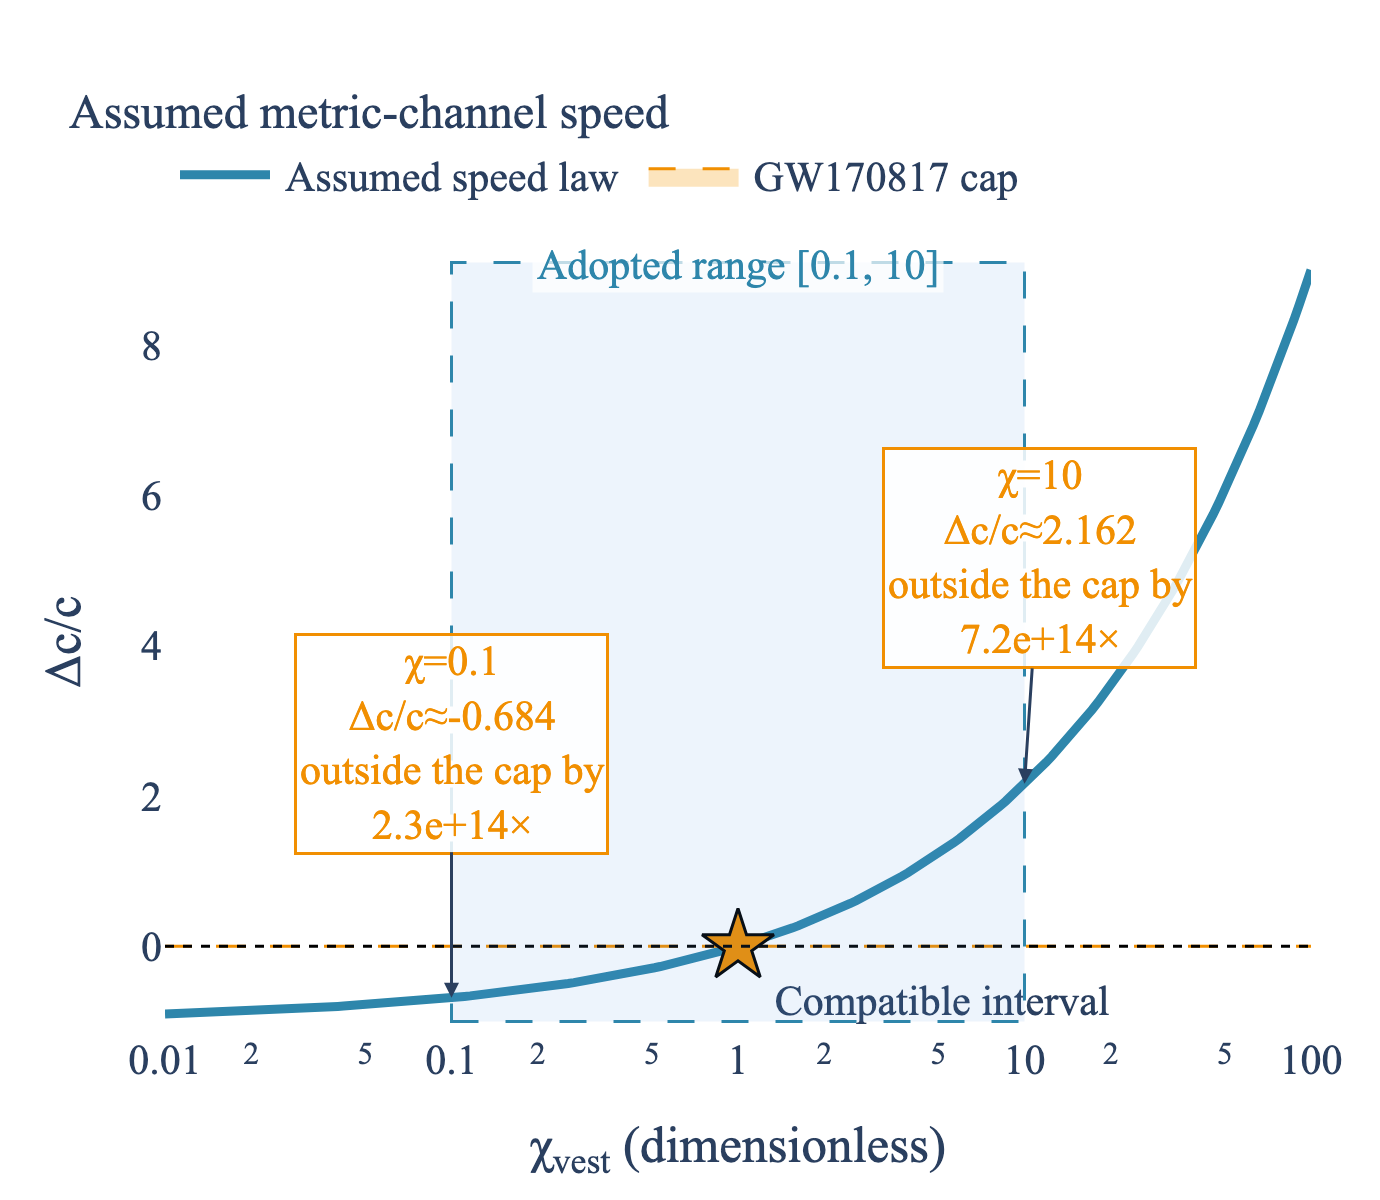
\includegraphics[width=0.96\columnwidth]{figures/fig_c_GW_vs_ligo_constraint.png}
\caption{Conditional speed-law constraint: $\dccap$ deviation across the
adopted $\chivest$ range, versus the GW170817 multi-messenger cap.
The amber band $|\dccap| \leq 3\times 10^{-15}$ is essentially
invisible at this scale. The adopted range $[0.1, 10]$ produces
$\dccap \in [-0.68, +2.16]$; both endpoints fail GW170817 by
$\sim 2.3\times10^{14}$ and $\sim 7.2\times10^{14}$,
respectively. The GW170817-compatible $\chivest$ window
$[(1-\tau)^{2},(1+\tau)^{2}]$ has finite width $4\tau$,
unresolved at this scale. The gold star marks its anchor
$\chivest=1$, not a singleton compatible set. Lean:
\texttt{vestigial\_natural\_range\_violates\_ligo}.}
\label{fig:cGW}
\end{figure}

Figure~\ref{fig:cGW} shows the deviation function
$\dccap(\chivest)$ over $\chivest \in [10^{-2}, 10^{2}]$ on
log-$\chivest$ axis with the adopted range
$[0.1, 10]$ highlighted. The GW170817 amber band is
unresolved around $\dccap=0$ at this scale. The plotted endpoint
offsets are of order unity; the more-than-fourteen-order width
comparison follows from the exact interval algebra, not pixel resolution.

%% ================================================================
\section{Discussion}
\label{sec:discussion}

\subsection{What this rules out}

Under the assumed leading-order law $\cGW=c\sqrt{\chivest}$,
the conservative symmetric cap requires
$\chivest\in[(1-\tau)^2,(1+\tau)^2]$. The susceptibility offsets
from unity are $-2\tau+\tau^2$ and $2\tau+\tau^2$,
approximately $\pm6\times10^{-15}$; the speed-deviation tolerance
is $\pm3\times10^{-15}$. Exact luminality occurs at $\chivest=1$,
but finite measurement tolerance permits the whole nonzero-width
interval. Its small relative width within $[0.1,10]$ alone neither
establishes a prior probability nor rules out generic UV theories
or requires an exact fixed point at unity.

\subsection{Open physical constructions}

A microscopic mechanism could constrain the metric-channel response
through a symmetry, identify a distinct propagating mode, or alter
the assumed frequency-independent speed law. The finite-tolerance
interval derives none of these possibilities and gives no reason
to prefer one. A symmetry selecting $\chivest=1$ would suffice,
but observational compatibility requires only the finite interval.
The illustrative correction in Sec.~\ref{sec:dispersion} remains
unmatched to a physical response; its placeholder cannot exclude
compensating corrections or establish a controlled frequency band.

\subsection{Comparison with the induced Newton coupling}

The companion study~\cite{Roehm2026LinearizedEFE} parameterizes
an induced Newton coupling by
$\GNemerg=\alpha_{\rm ADW}\,12\pi/(\Nf\,\Lambdauv^2)$.
Here $\Nf$ is the companion's fermion-species count parameter.
In units $\hbar=c=1$, write
$\Mpl=(G_{\rm N,obs})^{-1/2}$.
At the adopted cutoff $\Lambdauv=\Mpl$, exact matching requires
$\alpha_{\rm ADW}^{\star}=\Nf/(12\pi)$.
Its stated count choices give rounded matching values in
$[0.40,1.27]$, inside the adopted $[0.1,10]$ comparison interval.
The kernel's Dirac-count convention and these Weyl-count choices
require reconciliation before this supplies a physical Standard
Model normalization. The matching locus is conditional algebra;
it does not extract the microscopic coefficient selecting it.
That coefficient and $\chivest$ describe different response
normalizations. Neither adopted interval derives its physical value.

%% ================================================================
\section{Conclusions}
\label{sec:conclusions}

The scalar model $\cGW=c\sqrt{\chivest}$ gives an exact,
finite GW170817-compatible interval under the adopted conservative
cap. Its center, width, endpoint exclusions and prior dependence
are established mathematical consequences of the assumed law.
The formal tracked conjunction also has explicit counterexamples;
its scalar predicates do not construct a physical graviton.
The real-product frequency correction supplies conditional algebra,
not a physical transport coefficient or a measured band.

A physical realization requires the microscopic metric-channel
source and normalized susceptibility, a positive physical state,
a constrained propagating tensor mode relative to the same
matter/light reference, and controlled transport with units and
error bounds. Neither endpoint exclusion nor the narrow width
proves those constructions impossible. The comparison range $[0.1,10]$
is adopted in this calculation; deriving it remains a distinct
scientific obligation. No whole vestigial-branch exclusion follows.

%% ================================================================
\bibliographystyle{apsrev4-2}
\begin{thebibliography}{99}

\bibitem{Abbott2017GW170817} B.~P.~Abbott \emph{et al.}\
(LIGO Scientific Collaboration and Virgo Collaboration,
Fermi Gamma-ray Burst Monitor, and INTEGRAL),
``Gravitational Waves and Gamma-Rays from a Binary Neutron Star
Merger: GW170817 and GRB 170817A,''
Astrophys.\ J.\ Lett.\ \textbf{848}, L13 (2017);
arXiv:1710.05834.

\bibitem{Volovik2024Vestigial} G.~E.~Volovik, ``Fermionic Quartet
and Vestigial Gravity,'' JETP Lett.\ \textbf{119}, 330 (2024);
DOI: 10.1134/S002136402460006X.

\bibitem{Volovik2026SecondSound}
G.~E.~Volovik, ``Massless graviton in de Sitter as second sound in
two-fluid hydrodynamics,'' arXiv:2601.00639v1 (2026).

\bibitem{Volovik2022Counting} G.~E.~Volovik, ``Gravity from Symmetry
Breaking Phase Transition,'' J.\ Low Temp.\ Phys.\
\textbf{207}, 127 (2022); DOI: 10.1007/s10909-022-02694-z.

\bibitem{Vergeles2025} S.~N.~Vergeles, ``Unitarity of 4D Lattice
Theory of Gravity,'' Phys.\ Rev.\ D \textbf{112}, 054509 (2025);
arXiv:2506.00036.

\bibitem{Akama1978} K.~Akama, ``An Attempt at Pregeometry,''
Prog.\ Theor.\ Phys.\ \textbf{60}, 1900 (1978).

\bibitem{Diakonov2011} D.~Diakonov, ``Towards lattice-regularized
Quantum Gravity,'' arXiv:1109.0091v1 (2011).

\bibitem{HebeckerWetterich2003} A.~Hebecker and C.~Wetterich,
``Spinor gravity,'' Phys.\ Lett.\ B \textbf{574}, 269 (2003);
arXiv:hep-th/0307109.

\bibitem{Wetterich2022} C.~Wetterich, ``Spinor gravity and gauge
symmetry,'' JHEP \textbf{06}, 069 (2022); arXiv:2110.11138.

\bibitem{VladimirovDiakonov2012} A.~A.~Vladimirov and D.~Diakonov,
``Phase transitions in spinor quantum gravity on a lattice,''
Phys.\ Rev.\ D \textbf{86}, 104019 (2012); arXiv:1208.1254.

\bibitem{Roehm2026LinearizedEFE} J.~G.~Roehm, ``Linearized Einstein
Equations from Anderson--Higgs Tetrad Condensation,''
manuscript in preparation (2026).

\bibitem{CrossleyGloriosoLiu2017} P.~Crossley, P.~Glorioso, and
H.~Liu, ``Effective field theory of dissipative fluids,''
JHEP \textbf{09}, 095 (2017); arXiv:1511.03646.

\end{thebibliography}

\end{document}
